\documentclass[a4paper]{article} 
\addtolength{\hoffset}{-2.25cm}
\addtolength{\textwidth}{4.5cm}
\addtolength{\voffset}{-3.25cm}
\addtolength{\textheight}{5cm}
\setlength{\parskip}{0pt}
\setlength{\parindent}{0in}

%----------------------------------------------------------------------------------------
%	PACKAGES AND OTHER DOCUMENT CONFIGURATIONS
%----------------------------------------------------------------------------------------

\usepackage{blindtext} % Package to generate dummy text
\usepackage{charter} % Use the Charter font
\usepackage[utf8]{inputenc} % Use UTF-8 encoding
\usepackage{microtype} % Slightly tweak font spacing for aesthetics
\usepackage[english, ngerman]{babel} % Language hyphenation and typographical rules
\usepackage{amsthm, amsmath, amssymb} % Mathematical typesetting
\usepackage{float} % Improved interface for floating objects
\usepackage[final, colorlinks = true, 
            linkcolor = black, 
            citecolor = black]{hyperref} % For hyperlinks in the PDF
\usepackage{graphicx, multicol, subfigure} % Enhanced support for graphics
\usepackage{xcolor} % Driver-independent color extensions
\usepackage{marvosym, wasysym} % More symbols
\usepackage{rotating} % Rotation tools
\usepackage{censor} % Facilities for controlling restricted text
\usepackage{listings, style/lstlisting} % Environment for non-formatted code, !uses style file!
\usepackage{pseudocode} % Environment for specifying algorithms in a natural way
\usepackage{style/avm} % Environment for f-structures, !uses style file!
\usepackage{booktabs} % Enhances quality of tables
\usepackage{tikz-qtree} % Easy tree drawing tool
\tikzset{every tree node/.style={align=center,anchor=north},
         level distance=2cm} % Configuration for q-trees
\usepackage{style/btree} % Configuration for b-trees and b+-trees, !uses style file!
\usepackage[backend=biber,style=numeric,
            sorting=nyt]{biblatex} % Complete reimplementation of bibliographic facilities
\addbibresource{ecl.bib}
\usepackage{csquotes} % Context sensitive quotation facilities
\usepackage[yyyymmdd]{datetime} % Uses YEAR-MONTH-DAY format for dates
\renewcommand{\dateseparator}{-} % Sets dateseparator to '-'
\usepackage{fancyhdr} % Headers and footers
\pagestyle{fancy} % All pages have headers and footers
\fancyhead{}\renewcommand{\headrulewidth}{0pt} % Blank out the default header
\fancyfoot[L]{} % Custom footer text
\fancyfoot[C]{} % Custom footer text
\fancyfoot[R]{\thepage} % Custom footer text
\newcommand{\note}[1]{\marginpar{\scriptsize \textcolor{red}{#1}}} % Enables comments in red on margin

%----------------------------------------------------------------------------------------

\begin{document}

%-------------------------------
%	TITLE SECTION
%-------------------------------
\fancyhead[C]{}
\hrule \medskip % Upper rule
\begin{minipage}{0.295\textwidth} 
\raggedright
\footnotesize
Group Name: \hfill \\
Berkeley Goggles
\end{minipage}
\begin{minipage}{0.4\textwidth} 
\centering 
\large 
Project Question Solutions\\ 
\normalsize 
CS182\\ 
\end{minipage}
\begin{minipage}{0.295\textwidth} 
\raggedleft
\today\hfill\\
\end{minipage}
\medskip\hrule 
\bigskip
%-------------------------------
%	Problem
%-------------------------------
\section{Paper Introduction}
This homework explores Latent Diffusion Models as presented in the paper \href{https://arxiv.org/pdf/2112.10752.pdf}{High Resolution Image Synthesis with Latent Diffusion}. Diffusion models learn how to de-noise images that have had noise added to them during the diffusion process, which will be explored in this homework. Stable diffusion is a text conditional latent diffusion model, created by researchers and engineers from CompVis, Stability AI, and LAION. Diffusion models are incredibly expensive to the train so with the use of latent space, we can greatly reduce the computational resource requirements for training, and can also result in very competitive performance on tasks such as inpainting, text-to-image synthesis, super-resolution and more. We encourage you to read over the paper on your own as it is quite fascinating!

\subsection{Auto-encoders and Downsampling}
Latent diffusion models use pre-trained auto-encoders to produce a lower dimensional space representation of the input.
Auto-encoders downsample the input images by a factor of \(f=2^m, m  \, \epsilon \, \mathbb{R}\). The paper experiments with 6 different sampling factors \(f=[1, 2, 4, 8, 16, 32]\) abbrieviated as LDM-f. LDM-1 represents pixel-based diffusion models with no downsampling. The paper tested the performance on these 6 models and measured performance with two different scores: \href{https://en.wikipedia.org/wiki/Fr%C3%A9chet_inception_distance}{FID (Frechet Inception Distance)} which compares the distributions of images generated with the model and real images and \href{https://en.wikipedia.org/wiki/Inception_score}{IS (Inception Score)} which quantifies the quality of images generated by the model.

\begin{itemize}
    \item [(a)]
    Given two graphs that show the FID scores and IS scores against training progress, we can see that three of the LDM-f models perform well and three have weaker performance. Identify the top three performing LDM-f models and the bottom three performing LDM-f models. Provide a brief explanation for your answer.

     \begin{figure}[htbp]
        \centering
        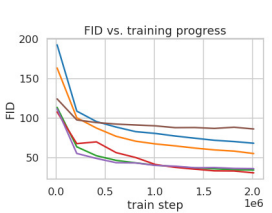
\includegraphics[width=0.4\textwidth]{fid_scores.png} \hfill
        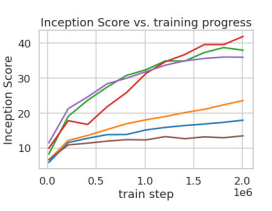
\includegraphics[width=0.4\textwidth]{is_scores.png}
        \caption{FID and IS Scores vs Training Progress}
        \label{fig:is}
    \end{figure}

\end{itemize}

\subsection{Conditional LDM Loss}
For a deeper explanation of the diffusion process, feel free to complete the code in Problem 2 first where an explanation of the diffusion process is provided in the Google Colab. We can think of diffusion models as a sequence of denoising auto-encoders \(\epsilon_{\theta}(x_t, t)\); \(t = 1...T\) where \(x_t\) is a noisy version of the input and  \(t\) is sampled uniformly.  We get the following loss for diffusion models:

\[L_{LDM} = \mathbb{E}_{\varepsilon(x), \varepsilon \sim \mathcal{N}(0, 1), t} [\| \varepsilon - \varepsilon_{\theta}(x_t, t) \|_2^2 ] \]

For a conditional LDM, we use a conditional denoising auto-encoder which takes in the latent representation, \(z_t\) and a domain specific encoder \(\tau_{\theta}\) that projects a text input \(y\) into an intermediate representation.  
\begin{itemize}
    \item [(b)]
    Write the loss function for a conditional LDM.
   
\end{itemize}

%-------------------------------
%	Problem
%-------------------------------
\section{Image Synthesis with Diffusion Model}

Please follow the instructions in this \href{https://colab.research.google.com/drive/1e_3xj1uvOjlD5duraQedHFuYNaiMwm8X?usp=sharing}{notebook}. 
You will implement a text conditioned denoising unet and the sampling algorithm. Then you'll see the diffusion process on a single image and try to train your own diffusion mode. Once you finished with the notebook,
\begin{itemize}
    \item download submission.zip and submit it to Gradescope.

    \item Answer the following questions in your submission of the written assignment:
\end{itemize}

\begin{itemize}
    \item [(a)]
    Why might a U-Net by a good choice for the model backbone? List two reasons.


    \item [(b)]
    Screenshot your visualization for get noisy image and include it in your submission of the written assignment. And describe the picture you observed briefly. What kind of process is this?


    \item [(c)]
    Screenshot one of your visualizations about the sampled images and include it in your submission of the written assignment. Then answer the following question. How does the model perform and does it meet your expectations? If not, what do you think are the directions for improvement?

    
\end{itemize}

%-------------------------------
%	Problem
%-------------------------------
\section{Understanding the VAE Loss}

Latent diffusion models use an autoencoder model similar to a VAE to encode images from pixel space to some compressed latent space, perform the diffusion process in this latent space, and finally decode the denoised latent back into pixel space. \\

To have our model learn the correct latent space, we would like the estimated posterior by the encoder \(q_{\phi}(z|x_{i})\) to be very close to the real posterior \(p_{\theta}(z|x_i)\). We can quantify this using the Kullback-Leibler (KL) divergence to get a measure of the difference between the two distributions, defined as 
\begin{center}
\(D_{KL}(P||Q) = \mathbb{E}_{x\sim P(x)}[log \frac{P(x)}{Q(x)}]\)
\end{center}

However, \(p_{\theta}(z|x_i)\) is intractable in practice. Another goal of VAE-like models is to maximize the probability of generating real samples, or \(p_{\theta}(x)\). During training, rather than directly maximizing this quantity, we maximize a lower-bound called the evidence lower bound (ELBO):
\begin{center}
\(log(p_{\theta}(x_i)) \ge \mathcal{L}(x_{i}, \theta, \phi) = \mathbb{E}_{z\sim q_{\phi}(z|x_{i})}[log(p_{\theta}(x_i | z)] - D_{KL}[q_{\phi}(z|x_{i}) || p_{\theta}(z)]\)
\end{center}
At a high-level, this loss can be seen as doing two things:
\begin{itemize}
    \item \textbf {Reconstruction loss}: The first term corresponds to the likelihood of generating images from the true data distribution given a sampled latent
    \item \textbf {Matching Prior}: The second term acts as a regularizer to minimize the difference between the estimated posterior and the prior (generally a standard normal).
\end{itemize}
Note: In the latent diffusion paper, the autoencoder loss is actually comprised of 3 terms: a patch-based discriminator loss for reconstruction, the standard KL-divergence term between \(q_{\phi}(z|x)\) and a prior \(p(z)\), and a regularizing term \(L_{reg}\) for the latent z to be zero centered and with small variance. For simplicity, however, we will just be analyzing the traditional ELBO loss here.
\begin{itemize}
    \item [(a)] \textbf {Show} that maximizing the ELBO loss also minimizes \(D_{KL}(q_{\phi}(z|x_{i})||p_{\theta}(z|x_i))\), the KL-divergence of the estimated posterior and the real posterior. \\\\
    \emph {Hint: Start with the KL-divergence formula and manipulate it to get ELBO loss plus some other term.}
    
\end{itemize}

\end{document}
